\documentclass[aspectratio=169,t,11pt]{beamer}
% License: MIT-Lizenz (https://opensource.org/licenses/MIT)
% Author: Bitcoin Entdecken / Bitcoin Austria

% Metropolis theme - Modern, minimalist Beamer theme
\usetheme[progressbar=foot]{metropolis}

% Bitcoin Entdecken style package
\usepackage{../styles/bitcoin-entdecken}

% Title information using Bitcoin Entdecken style helpers
\bitcointitle{Bitcoin}{Einfach erklärt}
\bitcointitlegraphic{pix/title.jpg}

\begin{document}

% Title slide
\begin{frame}
	\titlepage
\end{frame}

% Table of contents
\begin{frame}{Übersicht}
	\begin{itemize}
		\item Open Source
		\item Technische Geschichte
		\item Gewaltenteilung
		\item Was macht ein User
		      \begin{itemize}
			      \item Public-Key Cryptography (Adressen)
			      \item Generiert Adressen, verschickt Geld
		      \end{itemize}
		\item Was macht ein Node
		      \begin{itemize}
			      \item Validating, Messaging, Consensus
		      \end{itemize}
		\item Was macht ein Miner
		      \begin{itemize}
			      \item Generiert Bitcoin, Brute Forcing, Tic-Toc
		      \end{itemize}
	\end{itemize}
\end{frame}

\section{Open Source}

\begin{frame}{Closed Source vs. Open Source Software}
	\textbf{Closed Source} bedeutet:
	\begin{itemize}
		\item Bei den meisten Programmen ist der \textbf{Code nicht einsehbar}
		\item Man \textbf{vertraut} dem Entwickler blindlings
	\end{itemize}

	\vspace{0.5em}
	\textbf{Open Source} bedeutet:
	\begin{itemize}
		\item Code ist \textbf{verfügbar} und \textbf{überprüfbar}
		\item Programm kann von jedem \textbf{kompiliert} werden
	\end{itemize}

	\vspace{0.5em}
	\textbf{Bitcoin} funktioniert nur als \textbf{Open Source} Technologie

	\vspace{1em}
	\begin{alertblock}{\textcolor{white}{Grundsatz}}
		\vspace{3pt}
		\textbf{Vertrauen} ist gut, \textbf{Kontrolle} ist besser
		\vspace{3pt}
	\end{alertblock}
\end{frame}

\section{Gewaltenteilung}

\begin{frame}{Gewaltenteilung}
	\begin{columns}[T]
		\begin{column}{0.45\textwidth}
			\centering
			\textbf{Staatsgewalt}
			\vspace{1em}

			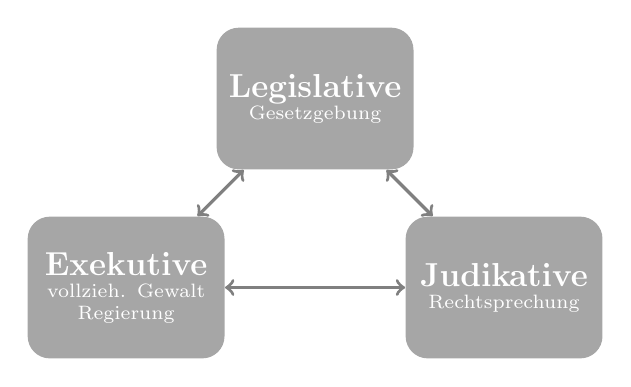
\begin{tikzpicture}[scale=0.8]
				% Legislative rounded rectangle
				\node[rectangle, rounded corners=8pt, fill=gray!70, text=white, minimum width=2.5cm, minimum height=1.8cm, font=\scriptsize, text width=2.2cm, align=center] (leg) at (0,3.0) {\textbf{\large Legislative}\\Gesetzgebung};

				% Judikative rounded rectangle
				\node[rectangle, rounded corners=8pt, fill=gray!70, text=white, minimum width=2.5cm, minimum height=1.8cm, font=\scriptsize, text width=2.2cm, align=center] (jud) at (3.0,0) {\textbf{\large Judikative}\\Rechtsprechung};

				% Exekutive rounded rectangle
				\node[rectangle, rounded corners=8pt, fill=gray!70, text=white, minimum width=2.5cm, minimum height=1.8cm, font=\scriptsize, text width=2.2cm, align=center] (exe) at (-3.0,0) {\textbf{\large Exekutive}\\vollzieh. Gewalt\\Regierung};

				% Arrows showing separation
				\draw[<->, gray, very thick] (leg) -- (jud);
				\draw[<->, gray, very thick] (jud) -- (exe);
				\draw[<->, gray, very thick] (exe) -- (leg);
			\end{tikzpicture}

			\vspace{0.5em}
		\end{column}

		\begin{column}{0.45\textwidth}
			\centering
			\textbf{Bitcoin}
			\vspace{1em}

			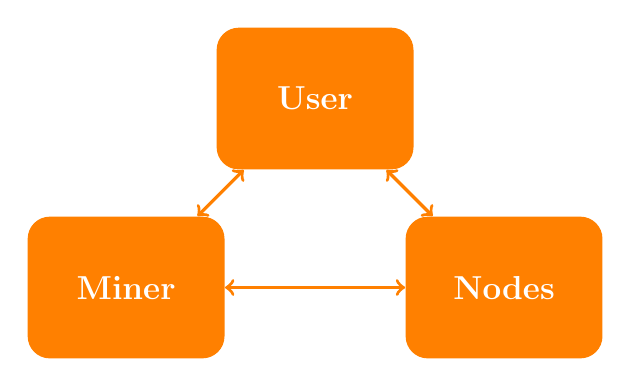
\begin{tikzpicture}[scale=0.8]
				% User rounded rectangle
				\node[rectangle, rounded corners=8pt, fill=orange, text=white, minimum width=2.5cm, minimum height=1.8cm, font=\scriptsize, text width=2.2cm, align=center] (user) at (0,3.0) {\textbf{\large User}};

				% Nodes rounded rectangle
				\node[rectangle, rounded corners=8pt, fill=orange, text=white, minimum width=2.5cm, minimum height=1.8cm, font=\scriptsize, text width=2.2cm, align=center] (nodes) at (3.0,0) {\textbf{\large Nodes}};

				% Miner rounded rectangle
				\node[rectangle, rounded corners=8pt, fill=orange, text=white, minimum width=2.5cm, minimum height=1.8cm, font=\scriptsize, text width=2.2cm, align=center] (miner) at (-3.0,0) {\textbf{\large Miner}};

				% Arrows showing interaction
				\draw[<->, orange, very thick] (user) -- (nodes);
				\draw[<->, orange, very thick] (nodes) -- (miner);
				\draw[<->, orange, very thick] (miner) -- (user);
			\end{tikzpicture}
		\end{column}
	\end{columns}

	\vspace{1em}
	\begin{alertblock}{\textcolor{white}{Zweck der Gewaltenteilung}}
		\small
		Beide Systeme trennen Macht auf verschiedene Akteure auf, um Machtmissbrauch zu verhindern und ein Gleichgewicht der Kräfte zu schaffen.
	\end{alertblock}
\end{frame}

\section{User}

\begin{frame}{User}
	\begin{columns}[T]
		\begin{column}{0.15\textwidth}
			\begin{tikzpicture}
				\node[circle, fill=bitcoinorange, text=white, minimum size=1.5cm, font=\huge] at (0,0) {₿};
				\node[below=0.3cm] at (0,-0.75) {\small User};
			\end{tikzpicture}
		\end{column}

		\begin{column}{0.8\textwidth}
			Verwendet Computer Code und erstellt einen zufälligen Privaten Schlüssel.\\
			Am Computer selbst nicht online.

			\vspace{1em}
			Berechnet daraus den zugehörigen Öffentlichen Schlüssel.

			\vspace{1em}
			Mit dem Privaten Schlüssel kann ich beweisen das mir der öffentliche Schlüssel gehört.

			\vspace{1em}
			Der User teilt jemandem den öffentlichen Schlüssel seiner Adresse mit und schickt an diese Adresse Bitcoin.
		\end{column}
	\end{columns}
\end{frame}

\section{Node}

\begin{frame}{Node}
	\begin{itemize}
		\item \textbf{Validating} - Überprüft alle Transaktionen und Blöcke
		\item \textbf{Messaging} - Kommuniziert mit anderen Nodes
		\item \textbf{Consensus} - Einigt sich mit anderen Nodes über gültige Regeln
	\end{itemize}
\end{frame}

\section{Miner}

\begin{frame}{Miner}
	\begin{itemize}
		\item \textbf{Generiert Bitcoin} - Erstellt neue Bitcoin durch Mining
		\item \textbf{Brute Forcing} - Sucht durch Ausprobieren nach gültigen Hashes
		\item \textbf{Tic-Toc} - Sorgt für regelmäßige Blockzeiten (~10 Minuten)
	\end{itemize}
\end{frame}

\section{Bitcoin Blöcke}

\begin{frame}{Bitcoin Blöcke}
	\begin{center}
		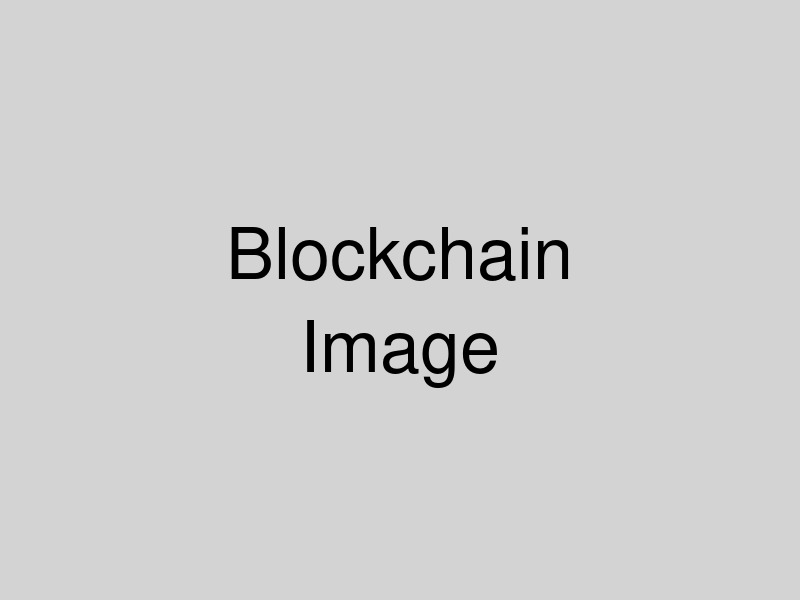
\includegraphics[width=0.9\textwidth,height=0.7\textheight,keepaspectratio]{pix/blockchain.jpg}
	\end{center}
\end{frame}

\section{Bitcoin Updates}

\begin{frame}{Bitcoin Updates}
	Werden nur dann adaptiert wenn fast alle Teilnehmer dafür sind

	\vspace{2em}

	\textbf{User} (sonst verlieren diese Vertrauen und verkaufen ihre Bitcoin)

	\vspace{1em}

	\textbf{Nodes} (sonst updaten diese nicht zu den neuen Regeln)

	\vspace{1em}

	\textbf{Miner} (sonst machen diese keinen Profit)

	\vspace{2em}

	\begin{tikzpicture}[remember picture,overlay]
		\node[anchor=south east] at ([xshift=-1cm,yshift=1cm]current page.south east) {
			
\includegraphics[width=3cm]{pix/update.jpg}
		};
	\end{tikzpicture}
\end{frame}

\section{Zusammenfassung}

\begin{frame}{Zu wenige Fragen und noch Zeit?}
	\begin{itemize}
		\item Schauen wir uns einmal einen Block an

		      \vspace{2em}

		\item Wie funktioniert die Ausgabe neuer Bitcoin

		      \vspace{2em}

		\item Wie sieht eine Transaktion im Detail aus
	\end{itemize}
\end{frame}

\end{document}
